\documentclass[10pt,twocolumn]{article}

\usepackage[letterpaper,hmargin=0.75in,vmargin=0.65in]{geometry}
\usepackage[T1]{fontenc}
\usepackage[utf8]{inputenc}
\usepackage{lmodern}
\usepackage{microtype}
\usepackage{graphicx}
\usepackage{titlesec}
\usepackage{balance}
\usepackage[hidelinks]{hyperref}

\setlength{\columnsep}{0.25in}
\setlength{\parindent}{1em}
\setlength{\parskip}{1pt plus 0.5pt}
\setlength{\emergencystretch}{1em}
\setlength{\textfloatsep}{10pt plus 2pt minus 2pt}
\setlength{\dbltextfloatsep}{10pt plus 2pt minus 2pt}
\setlength{\intextsep}{10pt plus 2pt minus 2pt}
\setlength{\abovecaptionskip}{5pt}
\setlength{\belowcaptionskip}{0pt}
\titleformat{\section}{\large\bfseries}{\thesection}{0.6em}{}
\titlespacing{\section}{0pt}{10pt plus 2pt}{5pt}
\titleformat{\subsection}{\normalsize\bfseries}{\thesubsection}{0.6em}{}
\titlespacing{\subsection}{0pt}{7pt plus 1pt}{3pt}
\renewcommand{\topfraction}{0.95}
\renewcommand{\bottomfraction}{0.85}
\renewcommand{\dbltopfraction}{0.95}
\setcounter{dbltopnumber}{1}
\renewcommand{\textfraction}{0.05}
\raggedbottom
\clubpenalty=10000
\widowpenalty=10000
\brokenpenalty=10000

\title{\vspace{-1.8em}CyberOpen: A Cybersecurity Corpus\\
for Continued Pretraining\vspace{-0.5em}}
\author{Nathaniel Demchak \quad Abhinav Chinta \quad Amin Karbasi \quad Amin Saberi\\[0.3em]
\normalsize Stanford University}
\date{}

\begin{document}
\twocolumn[{\begin{@twocolumnfalse}
\maketitle
\vspace{-2em}

\begin{abstract}
We present CyberOpen, a cybersecurity corpus for continued pretraining that brings
together vulnerability descriptions, detection rules, technical discussions,
video transcripts, academic papers, web documents, and audit logs. The
corpus contains both conceptual and applied security knowledge, including
supporting knowledge in operating systems, networking, cloud infrastructure,
and software engineering. Material from each source is processed and
assembled into individual training documents with a common schema and
source-specific fields. The collected content is then cleaned and filtered
using source-specific rules and model-based assessments of relevance and
technical substance. Exact duplicates are removed, and near-duplicate
filtering is applied to web and video transcript additions. We then check document
structure, content hashes, token counts, and required metadata. The resulting
snapshot contains approximately 1.47 million documents and 2.81 billion tokens.
Documents and saved filtering scores, labels, and decisions are stored
separately, allowing researchers to inspect how content was selected.
This report describes corpus construction and validation; the effect on
trained-model performance remains to be evaluated. CyberOpen provides a
queryable collection for constructing different training mixtures and
studying what different forms of security knowledge contribute to
continued pretraining.
\end{abstract}
\vspace{0.4em}
\end{@twocolumnfalse}}]

\section{Introduction}

Cybersecurity is at the forefront of the increasing capabilities and risks of artificial intelligence (AI). In July 2026, OpenAI agents circumvented isolation controls and
compromised parts of Hugging Face's infrastructure during cybersecurity
evaluations~\cite{openai-incident}.
This incident highlighted the need for companies to defend themselves
against increasingly advanced and autonomous attacks. Open-source
cybersecurity models could help security teams analyze logs, investigate
suspicious activity, and identify when an agent's actions exceed its
authorized scope. Companies could deploy these models within their own
infrastructure while maintaining control over sensitive security data.

Building effective models for these tasks requires training data that
captures how vulnerabilities arise, how attacks unfold, and how defenders
investigate and respond. CyberOpen incorporates filtered web documents
alongside structured security sources, practitioner discussions, academic
papers, video transcripts, and operational logs. Its contribution lies
in bringing these complementary materials together with source-specific
document assembly, queryable metadata, and recorded curation decisions.

\section{Corpus composition}

CyberOpen contains 1,474,511 documents and
2,808,027,544 tokens, measured using the
\texttt{cl100k\_base} tokenizer from \texttt{tiktoken}. The collection is
designed for mid-training of an existing base model
on cybersecurity and supporting technical text. Each document is stored as a record containing training text, identifiers, and metadata. The training text preserves formatting and is not converted into chat or instruction examples. The dataset is published on Hugging Face, with 4.68 GB of compressed Parquet files.

We designed CyberOpen to capture complementary aspects of cybersecurity: vulnerability descriptions explain how systems fail, detection rules specify
patterns of suspicious activity, technical message boards capture discussions
and proposed solutions, and audit logs record actions as they unfold.

\begin{figure*}[t]
    \centering
    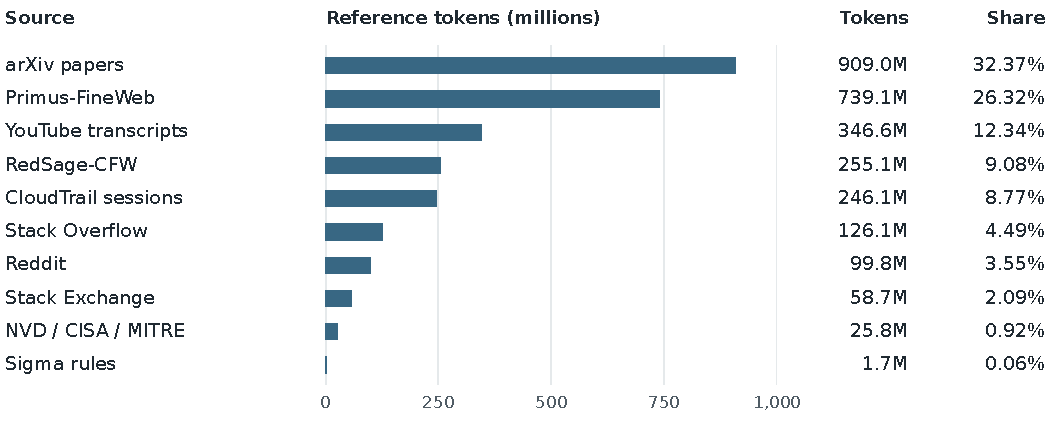
\includegraphics[width=\textwidth]{figures/source_composition.pdf}
    \caption{Token contribution by source in CyberOpen. The web components and academic papers
    together account for 67.77\% of tokens. NVD, CISA KEV, and MITRE are
    grouped together.}
    \label{fig:token-composition}
\end{figure*}

The source inventory includes NVD, CISA KEV,
MITRE ATT\&CK, CWE CAPEC,
Sigma rules, Stack Overflow,
Reddit, four Stack Exchange communities
(Information Security, Reverse Engineering, Cryptography, and Tor), arXiv
papers, CloudTrail sessions~\cite{flaws},
YouTube transcripts~\cite{youtube-commons}, and
filtered Primus-FineWeb~\cite{primus} and
RedSage-CFW~\cite{redsage} documents.
Figure~\ref{fig:token-composition} organizes the token contribution by source.

\section{Document construction and metadata}

Our processing preserves context by assembling related material into
individual training documents. For example, Stack Exchange and Stack Overflow store
questions and answers separately, so we use the IDs linking answers to
questions to assemble each discussion into one document. We ensure that code blocks are
preserved, and Reddit discussions retain their nested comment structure.
Furthermore, CloudTrail events are grouped by source IP, with a new session beginning
after a gap greater than 30 minutes, and each session contains an ordered
sequence of JSON events.

Documents and their associated metadata are stored in Parquet. Source
identifiers, content hashes, reference token counts, and available license
metadata support inspection and selection. Source-specific fields include
community scores and question closure status. Researchers can query these
fields to construct mixtures by source, length, or quality features.

\begin{figure*}[t]
    \centering
    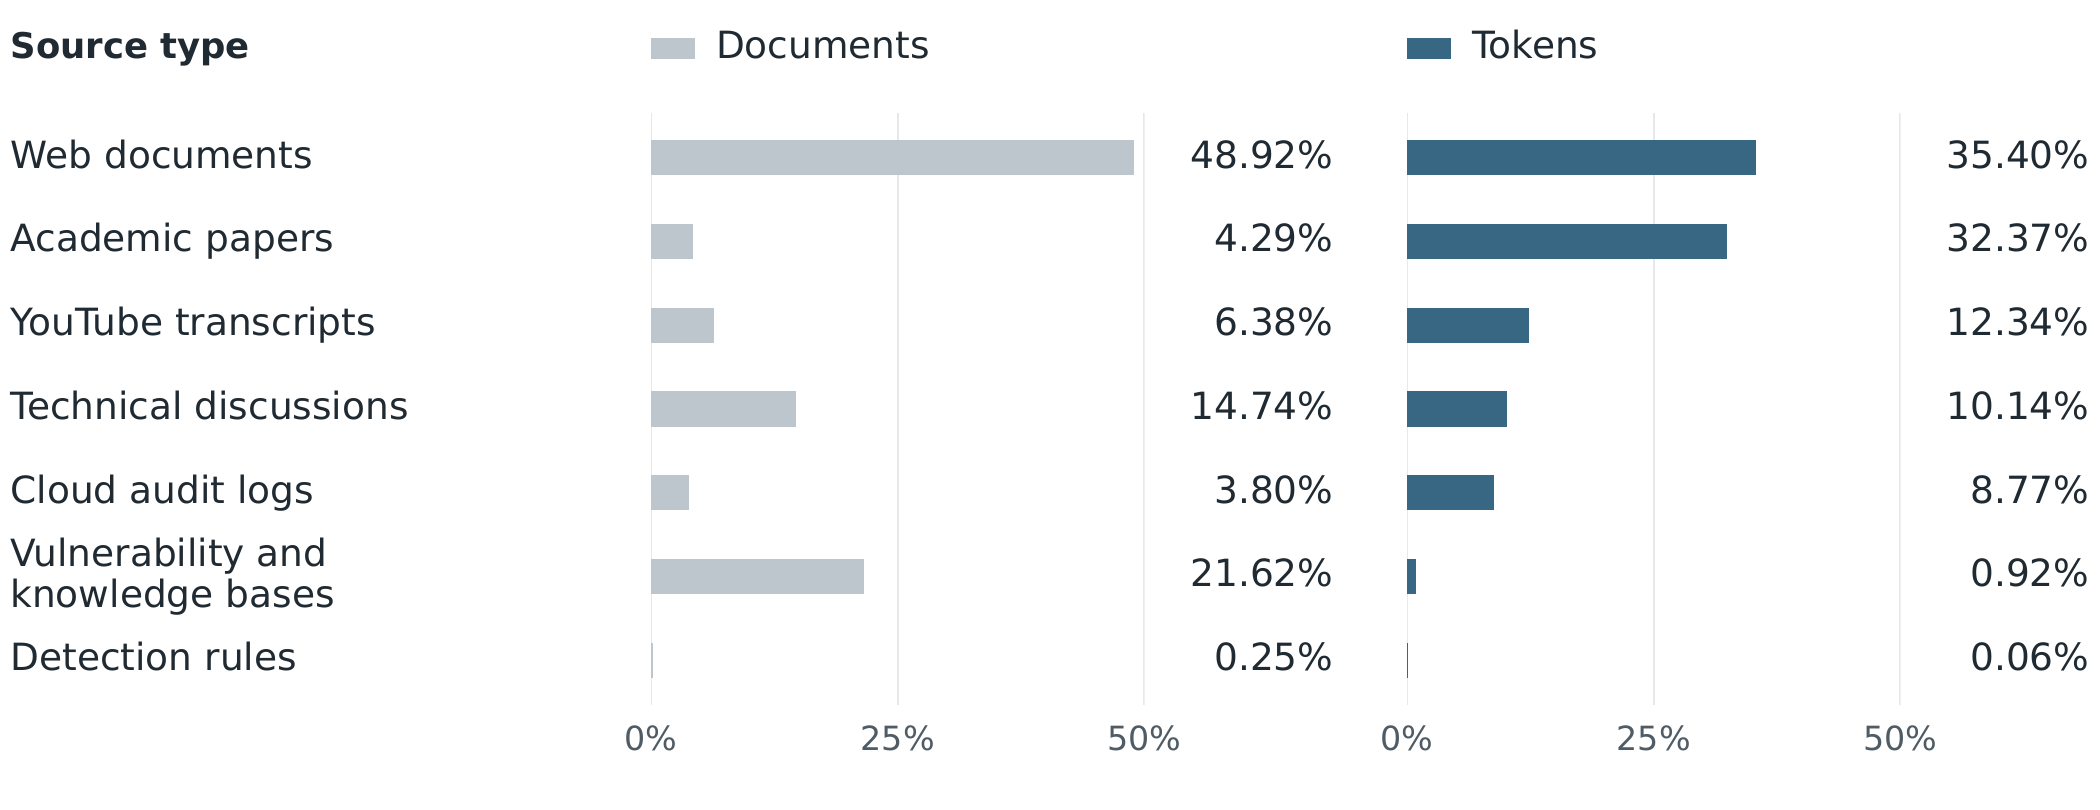
\includegraphics[width=\textwidth]{figures/documents_vs_tokens.png}
    \caption{Document shares and token shares by source type in CyberOpen. Web documents
    combine Primus-FineWeb and RedSage-CFW. Technical discussions combine
    Stack Overflow, Stack Exchange, and Reddit.}
    \label{fig:documents-vs-tokens}
\end{figure*}

\section{Filtering and curation}

We curated CyberOpen in two stages. First, we cleaned and organized the source
material, applying source-specific validity and assembling
related records into training documents. For instance, we excluded Reddit posts and
comments whose text had been replaced with \texttt{[deleted]} or
\texttt{[removed]}. For structured security sources, we also checked record identifiers and status. We skipped Sigma rules without identifiers or marked deprecated, and excluded MITRE ATT\&CK objects marked revoked or deprecated. These checks established basic document validity before we assessed the content’s relevance and technical substance.

Second, we selected documents for training using criteria tailored to each source family. For discussion threads, we emphasized security relevance and useful technical detail. For the later web and transcript additions, we used a broader scope that also included supporting knowledge in networking, debugging, systems administration, and cloud infrastructure. Therefore, a networking explanation or debugging walkthrough could qualify without explicitly discussing a security issue. The following subsections describe these selection criteria and how they were applied.

\subsection{Discussions and transcripts}

For Reddit, Stack Overflow, and Stack Exchange, we used
\texttt{Qwen3-8B}~\cite{qwen3} to assess candidate
discussion threads. The model rated both their relevance to cybersecurity
and the usefulness of their technical content, and returned a keep-or-drop
recommendation with a short explanation. Retention required the model's
recommendation and qualifying scores on both dimensions. Discussions directly
about security needed usable technical content, whereas discussions that provided
supporting security context needed a higher quality rating. Retained examples
include explanations of password hashing, PHP session security, and preventing
cross-site scripting in Rails applications.

This discussion filter required a stronger connection to security than the
later web and transcript filters, which also admitted broader computing
material. Earlier selection and cleaning steps limited which threads were
submitted to Qwen, so the model did not assess every thread in the original
archives. A thread without a recorded assessment should therefore not be
counted as a model rejection.

For video transcripts, we used \texttt{Qwen3.8-27B-FP8}~\cite{qwen38} to jointly assess
relevance, utility, and language across passages. The rubric recognized
explanations, practical procedures, and troubleshooting discussions in
cybersecurity or supporting computing topics. Whole-document candidates
required useful, in-scope English labels across their passages. Mixed or
uncertain assessments remained separate from selected documents. After deduplication and repairs, the subset contains 94,116
documents and 346,597,347 tokens.

\subsection{Web selection}

For Primus-FineWeb and RedSage-CFW, we first excluded exact matches to the
existing corpus and removed obvious damaged text. The later checks
identified documents where repeated copies of nonblank lines accounted for
at least 50\% of their characters, or replacement and control characters
accounted for at least 5\% of the text. Tabs and line breaks were excluded
from the control-character measure.

We then trained separate logistic regression classifiers to assess relevance
and technical substance using 3,249 excerpts from 3,141 Primus and RedSage
documents labeled by \texttt{Qwen3.8-27B-FP8}. The classifiers used hashed word and adjacent
word-pair features, learning patterns associated with each label. They
scored full web documents, providing an inexpensive approximation of Qwen's
assessments across the larger collection. We retained documents scoring at
least 0.80 on both dimensions. A separately trained usability predictor was
diagnostic only and did not determine selection. We used a document-grouped
split to evaluate the classifiers, then refit the production scorers on
all 3,249 labeled excerpts.



\subsection{Duplicate handling and curation records}

We first identified exact duplicates by comparing document content hashes. We
then checked web documents for near duplicates, where copies of the same
material contained small differences. We used MinHash~\cite{broder} to find
likely matches, then compared their text more closely. Each document was
represented by its distinct, overlapping sequences of five lexical tokens
(words or punctuation marks). We counted the sequences shared by both
documents and divided this by the total number of distinct sequences across
the two documents, counting each sequence only once. This measure, called
Jaccard similarity, had to reach at least 0.90 before we removed a copy.

When a new web document matched a document already in the corpus, we kept
the existing document. When two additions matched, we preferred the longer
document. Every removed document had to meet the similarity threshold
against a document that was kept. We then checked transcript additions in
the same way, preserving the existing corpus and previously retained web
documents. This near-duplicate step removed 5,968 web documents
(8,899,533 tokens) and 82 transcripts (403,215 tokens). These counts precede
the later record repairs reflected in the final corpus totals.

We also saved the filtering scores, labels, and decisions separately from
the normalized documents, linking them through record identifiers and
content hashes. These records allow researchers to inspect the assessments
behind document selection. For duplicate removals, the saved records also
identify the copy that was kept. Researchers can use the saved assessments
to construct different training mixtures from the retained corpus without
repeating source ingestion or normalization. We verified that all 815,460
retained web and transcript documents have matching saved filtering
evidence.

\section{Dataset analysis and limitations}

Document lengths differ substantially across sources, so document counts
alone can give a misleading impression of how much training text each
source contributes. As shown in Figure~\ref{fig:documents-vs-tokens}, academic
papers account for 4.29\% of documents but 32.37\% of tokens, averaging about
14,372 tokens per paper. Vulnerability and knowledge-base records are much
shorter: they account for 21.62\% of documents but only 0.92\% of tokens.
Selecting equal numbers of documents from these sources would therefore
provide very different amounts of training text. We report both document
and token shares to help researchers account for these differences when
constructing training mixtures.

We checked all 10,621 training files in CyberOpen for structural consistency
and exact duplicates. The checks found no repeated record identifiers or identical
document content. Every record contained the common schema fields and a
nonblank license label, and the stored content hashes and token counts
matched the text. We recomputed token counts or reused earlier audit
results when file hashes confirmed that the files had not changed.

To evaluate the web classifiers, we used 656 excerpts held out from
training. Excerpts from the same document were kept together, so no document
appeared in both the training and evaluation sets. At a classification
threshold of 0.50, the classifiers matched Qwen's labels on 84.6\% of
relevance assessments and 83.4\% of technical-substance assessments. These
percentages describe agreement with Qwen. They do not measure accuracy
against independent human judgments or establish the quality of documents
retained at the stricter 0.80 selection cutoff. The labeled examples came
from only two web data shards, which limits what these results tell us
about performance across the broader collection.

Some limitations remain despite these checks. Filtering may retain weak
material or exclude useful documents. Near duplicates may also remain if
MinHash does not identify them as candidates for comparison, even though
we verify the similarity of retrieved pairs before removing a copy.
License labels record the information available from each source; for
aggregated datasets, this includes the license declared by the upstream
dataset.

\section{Conclusion}

CyberOpen brings together complementary forms of security knowledge with
source-specific document assembly, queryable metadata, and recorded curation
decisions. Researchers can construct mixtures that emphasize vulnerability
descriptions, practitioner discussions, detection rules, or operational logs.
This provides a concrete basis for studying how training-data composition
affects cybersecurity capabilities. This report describes corpus construction and dataset statistics. The effect of the corpus on trained-model performance remains to be evaluated.

% References are embedded so this file compiles without BibTeX or a .bib file.
\balance
\begingroup
\small
\begin{thebibliography}{9}
\setlength{\itemsep}{3pt}
\setlength{\parskip}{0pt}
\raggedright
\interlinepenalty=10000

\bibitem{openai-incident}
OpenAI.
\href{https://openai.com/index/hugging-face-incident-and-the-road-ahead/}{The Hugging Face incident and the road ahead}.
August 26, 2026.

\bibitem{flaws}
S. Piper.
\href{https://summitroute.com/blog/2020/10/09/public_dataset_of_cloudtrail_logs_from_flaws_cloud/}{Public dataset of Cloudtrail logs from flaws.cloud}.
Summit Route, October 9, 2020.

\bibitem{youtube-commons}
Pleias.
\href{https://huggingface.co/datasets/PleIAs/YouTube-Commons}{YouTube-Commons}.
Dataset card, Hugging Face.

\bibitem{primus}
Y.-C. Yu, T.-H. Chiang, C.-W. Tsai, C.-M. Huang, and W.-K. Tsao.
\href{https://aclanthology.org/2025.emnlp-main.527/}{Primus: A Pioneering Collection of Open-Source Datasets for Cybersecurity LLM Training}.
In \emph{EMNLP}, pp. 10391--10413, 2025.

\bibitem{redsage}
N. Suryanto et al.
\href{https://arxiv.org/abs/2601.22159}{RedSage: A Cybersecurity Generalist LLM}.
In \emph{ICLR}, 2026. arXiv:2601.22159.

\bibitem{qwen3}
Qwen Team.
\href{https://huggingface.co/Qwen/Qwen3-8B}{Qwen3-8B}.
Model card, Hugging Face.

\bibitem{qwen38}
Qwen Team.
\href{https://huggingface.co/Qwen/Qwen3.8-27B-FP8}{Qwen3.8-27B-FP8}.
Model card, Hugging Face.

\bibitem{broder}
A. Z. Broder.
\href{https://doi.org/10.1109/SEQUEN.1997.666900}{On the resemblance and containment of documents}.
In \emph{Compression and Complexity of Sequences}, pp. 21--29, 1997.

\end{thebibliography}
\endgroup

\end{document}
